\usepackage{cleveref}
\subsection{Identity Provider}
\label{identity-provider}

To achieve persistent user identities in Graffiti
we use the Solid OpenID Connect specification~\cite{solid-oidc}.
On the surface level, this provides Graffiti applications
with an single-sign-on interface akin to a "Sign In with Google" button
as shown in Figure~\ref{fig:solid-oidc}.
However, while most single-sign-on interfaces only authorize
the client application to interface with a single server,
Solid OIDC authorizes the client application
to communicate with any server on the user's behalf which
is necessary for users to pull data from the multiple storage pods
we describe in~\cref{storage-pods}.
Additionally, the user can choose from any compliant
Solid identity provider including one they host themselves.

\begin{figure}
\label{fig:solid-oidc}
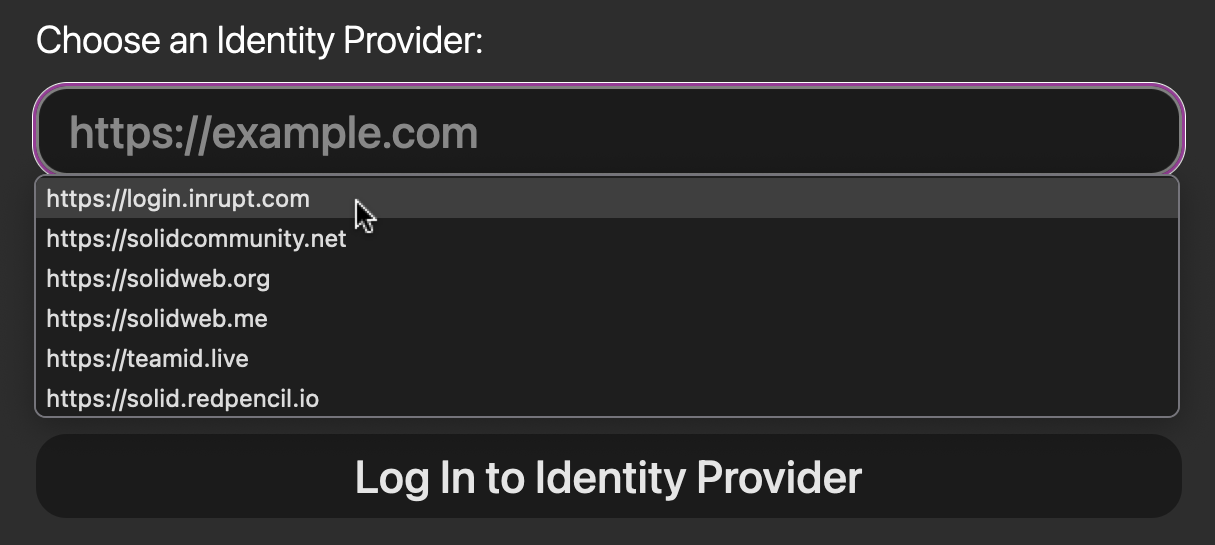
\includegraphics{paper/system/solid-oidc.png}
\caption{A user can choose from several common Solid identity providers
or manualy enter a custom one.}
\end{figure}

The Solid OIDC specification also provides
each user with a webId, a globally unique and human-readable URL
that can be shared like a username or an email address.
At this URL, the user can store a small amount of public data
which we use to implement "delegation".

There are multiple open source implimentations of Solid OIDC servers,
client libraries, and authorization libraries that we use out of the box.
While these implimentations were useful for getting started,
they have some limitations that we would eventually like to address.
None of thse limiations are necessarily at odds with the Solid OIDC
specification, they are either not implemented in the current libraries
or not fully laid out in the specification.

For one, the most popular browser client library is quite large
because it includes other Solid semantic web features not relevant to Graffiti.
This leads to large bundle sizes that can be slow and make Graffiti inaccessable
to users with limited data plans.

Additionally, existing OIDC servers generate their own
webIds, which are often verbose,
\emph{e.g.} \url{janedoe.solidcommunity.net/profile/card#me}.
There is no reason why a user could not come with their own, simple, domain name, for example
\url{id.janedoe.com}, similar to the AT Protocol~\cite{bluesky}. This would also give the users the ability
to switch identity providers while maintaining their identity.
It is not also currently easy to generate throwaway webIds
which could be useful for one-time or anonymous interactions.

Finally, once you are logged in with a webId users are
granted full access rights. Incorporating scoped access rights
into the Solid OIDC specification would allow users to comfortably
interact with new applications without the risk of exposing or losing
their data.
